\documentclass{aa}

\usepackage{graphicx}

\usepackage{txfonts}

\usepackage[hidelinks]{hyperref}

\usepackage{amsmath}

\usepackage{float}

\graphicspath{{./figs/}}

\usepackage{verbatim}

\begin{document} 


   \title{CHEOPS Mission Reduction Pipeline Development}

   \subtitle{Simulation of WASP-18 b - Visit 2}

   \author{João P. S. Rodrigues}

   \institute{Departamento de Física e Astronomia da Universidade do Porto \\
              \email{up201405201@fc.up.pt}              
             }

   \date{}

% \abstract{}{}{}{}{} 
% 5 {} token are mandatory
 
  \abstract
  % context heading (optional)
  % {} leave it empty if necessary  
   {}
  % aims heading (mandatory)
   {}
  % methods heading (mandatory)
   {}
  % results heading (mandatory)
   {}
  % conclusions heading (optional), leave it empty if necessary 
   {}

   \keywords{}

   \maketitle
%
%________________________________________________________________

\section{Introduction}
%__________________________________________________________________

\section{Overscan}

The first step in treating the data is to subtract the overscan values from the image in order to remove the so-called Bias - a systematic error such as electronic noise introduced while reading the CCD .

\begin{figure}[H]
\centering
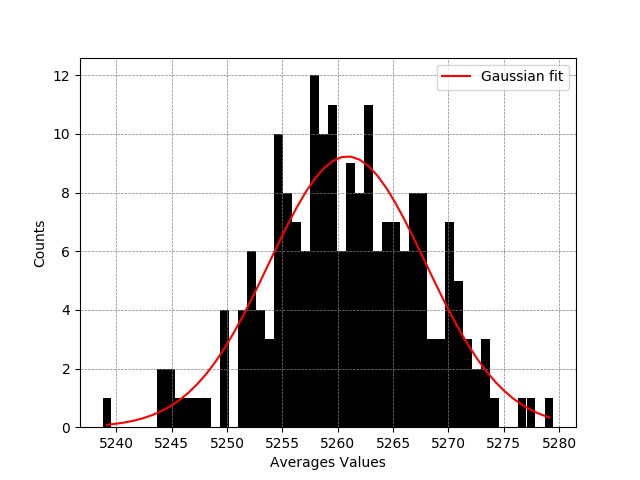
\includegraphics[width=.4\textwidth]{overscan_hist.png}
\caption{Histogram of averages for each line of the 4 columns.}
\label{fig:overscan_hist}
\end{figure}

Since each image is provided with four extra columns of overscan wich contain no data appart from the reading noise, we can use these columns to compute the overscan. By performing an average over each line of the columns and computing the histogram of these average values, we can approximate the noise with a gaussian curve (see Fig. \ref{fig:overscan_hist}). The fit was optimized using the least squares method and the final parameters are $[A, \mu , \sigma] = [9.23, 5260.86, 7.07]$ with one standard deviation errors of $[0.515, 0.455, 0.457]$ respectively.

This allows us to perform an average over all of the four columns and subtract that value from the image data, without introducing significant error.

\section{Flat Field}

The next critical step of the reduction pipeline is to account for the imperfections of the CCD screen when acquiring data. This is done by capturing what is called a Flat Field (FF) image which is the data aquired by the sensor when pointed at a uniform screen.

In order to remove this inconsistent data, the captured images must be divided by the data in the FF image, resulting in an image in which all the CCD pixels have roughly the same sensitivity.

After this step is performed, the pre-processing of the images is complete and one can begin computing the area of the image wherein the target lies, with the objective of performing a photometric measurement.

\section{Center of Mass Calculation}

Taking into account that the order of the counts belonging to the target is much larger than in the rest of the image, one can assume that a rough approximation of the target's position is a computation of the image's center of mass.

However, by computing the center of mass of the whole image, we find that it's position varies in a circular way. This is due to the rotation of the satellite together with the other objects which very faintly appear in the images. These objects are better observed by computing a convolution of the image with a Scharr Kernel of the type:

\begin{equation}
\begin{bmatrix}

-3-3j  & 0-10j &  +3 -3j \\
-10+0j & 0+ 0j & +10 +0j \\
-3+3j  & 0+10j &  +3 +3j

\end{bmatrix}
\end{equation}

which computes the gradient of the image both in magnitude and direction. The direction of the image's gradient is shown in Fig. \ref{fig:gradient_cm} (a) where the existence of at least three other objects, besides the target, is made obvious. We can also notice that these objects are rotating around the target in a clockwise manner which explains the circular movement of the images' center of mass, seen in Fig. \ref{fig:gradient_cm} (b).

\begin{figure}
\centering

(a) 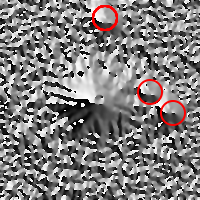
\includegraphics[width=.2\textwidth]{gradient_angle_img_0.png}
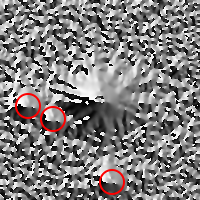
\includegraphics[width=.2\textwidth]{gradient_angle_img_45.png}

(b) 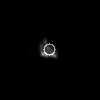
\includegraphics[width=.2\textwidth]{cm_r_100_img_0.png}
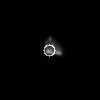
\includegraphics[width=.2\textwidth]{cm_r_100_img_45.png}

(c) 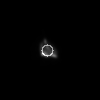
\includegraphics[width=.2\textwidth]{cm_r_20_img_0.png}
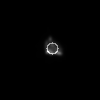
\includegraphics[width=.2\textwidth]{cm_r_20_img_45.png}
\caption{From top to bottom: (a) Direction of the images' gradient.
							  (b) Center of mass calculated using the whole image.
							  (c) Center of mass calculated using a square of size 20 pixels 									 centered on the images' center.}
\label{fig:gradient_cm}
\end{figure}

As a means to fix this problem, the center of mass was calculated using a square centered on the images' center and of a radius $r_{CM}$ to be empirically computed in Sec. \ref{sec:param_opt}. This way, the calculation only envolves the target and not the other objects, thus improving the stability of the center of mass, which can be seen in Fig. \ref{fig:gradient_cm} (c).

\section{Canny Edge Detection}

From observing the images in Fig. \ref{fig:gradient_cm} (a), an idea arised to use the gradient of the images to find the region on which to perform the photometry. An obvious candidate for an algorithm popped into mind: Canny Edge Detection \cite{canny}. The algorithm has the following steps:

\begin{enumerate}
\item Apply Gaussian filter to remove noise.
\item Compute intensity gradient of the image.
\item Apply non-maximum surpression.
\item Apply double threshold to determine edges.
\item Edge tracking by hysteresis.
\end{enumerate}

Even though this is the standard procedure to perform the canny edge algorithm, we can disregard the third step since applying the surpression is just an edge-thining technique which is of no use for us since we want to find the area inside the outer edges, anyway.

The same principle (used in the calculation of the center of mass) of applying the algorithm to a box centered on the image was utilized here in order to find only the edges of the target. As such, this algorithm, if correctly applied - using optimized parameters of filter $\sigma$ and double thresholds, discussed in Sec. \ref{sec:param_opt} - should return the area of the target in a specific image.

As can be seen in Fig. \ref{fig:img_0_canny}, the algorithm seems to be a good candidate for detecting the target's area, for as much as can be seen with the naked eye. This figure was obtained with $\sigma = 0.6$, higher threshold $T = 4000$ and lower threshold $t = 0.3T$.

\begin{figure}
\centering

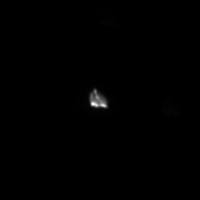
\includegraphics[width=.2\textwidth]{img_0.png}
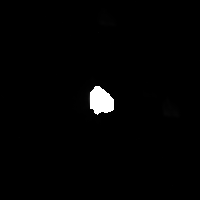
\includegraphics[width=.2\textwidth]{img_0_canny.png}

\caption{Comparison of image 0 target with detected area.}
\label{fig:img_0_canny}
\end{figure}

\section{Background Estimation}

In order to obtain an accurate result for the photometry, it is essencial that we account for the background counts present in the whole image. This value has to be estimated and subtracted from the image.

Firstly, since the image contains other light sources as seen above, the mode of the image should represent better the value of the background as opposed to the mean which should have a contribution from these other sources. Besides that, the target should not be considered in the calculation of the background and thus only points outside a square of side $r_{bkg}$ will be taken into account.

By calculating the mode for each of the images, we can see that it has an approximately sinusoidal variation (see Fig. \ref{fig:mode}) which can be fitted. The fit parameters and respective one standard deviation error are shown in Tab. \ref{tab:mode}.

\begin{table}
\caption{Mode sin fit parameters.}
\label{tab:mode}
\centering
\begin{tabular}{c c c}
\hline
\noalign{\smallskip}
Parameter & Value & $1\ \sigma$ \ error \\
\hline
\noalign{\smallskip}
	A & $8.14\ \mathrm{e}{+0}$      & $2.98\ \mathrm{e}{-1}$ \\
	f & $1.03\ \mathrm{e}{-2}$      & $4.64\ \mathrm{e}{-5}$ \\
	$\phi$ & $4.97\ \mathrm{e}{+1}$ & $6.89\ \mathrm{e}{-2}$ \\
	DC & $6.01\ \mathrm{e}{+1}$     & $2.07\ \mathrm{e}{-1}$
\end{tabular}
\end{table}

\begin{figure}[h]
\centering

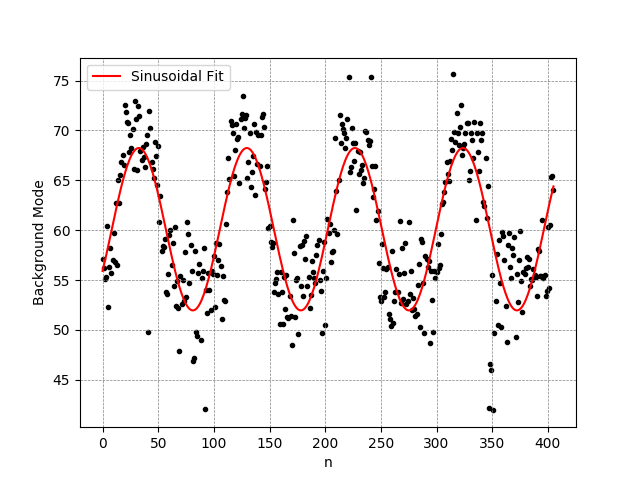
\includegraphics[width=.4\textwidth]{background_mode.png}

\caption{Background mode throughout the images.}
\label{fig:mode}
\end{figure}

From the sinusoidal fit, we can estimate the period of the mode oscillation to be $1/f = 97.03\ images$ which approximately corresponds to the period of rotation of the satellite, 100 minutes (since the integration time of the instrument is $1\ min$).

On the other hand, the mean of the background can also be calculated in order to account for random oscillations in the image, which are not, in general, captured by the mode. As can be seen in Fig. \ref{tab:mean}, the mean detects the passage of the telescope through the South Atlantic Anomaly, caracterized by random peaks of noise around images $90$ and $350$.

The same sinusoidal fit can be calculated for the mean data, using images in the range $[100-340]$. Tab. \ref{tab:mean} shows the parameters obtained in this calculation. The period of the sine wave is now $1/f = 97.43$ which is in close agreement with the result obtained from the mode.

\begin{table}
\caption{Mean sin fit parameters.}
\label{tab:mean}
\centering
\begin{tabular}{c c c}
\hline
\noalign{\smallskip}
Parameter & Value & $1\ \sigma$ \ error \\
\hline
\noalign{\smallskip}
	A & $8.78\ \mathrm{e}{+0}$      & $2.30\ \mathrm{e}{-1}$ \\
	f & $1.02\ \mathrm{e}{-2}$      & $6.03\ \mathrm{e}{-5}$ \\
	$\phi$ & $4.96\ \mathrm{e}{+1}$ & $8.47\ \mathrm{e}{-2}$ \\
	DC & $8.94\ \mathrm{e}{+1}$     & $1.64\ \mathrm{e}{-1}$
\end{tabular}
\end{table}

\begin{figure}
\centering

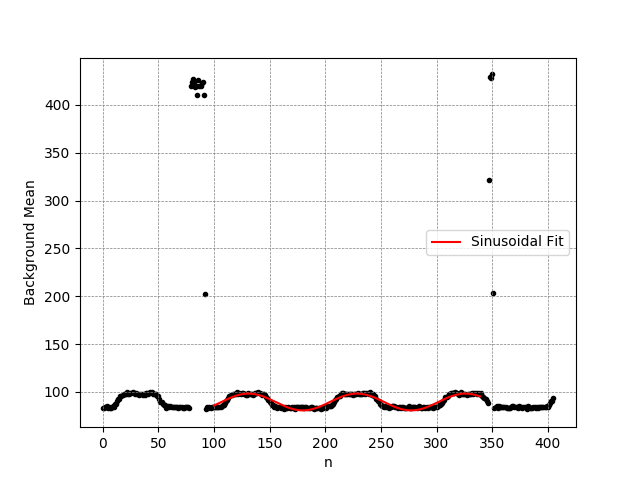
\includegraphics[width=.4\textwidth]{background_avg.png}

\caption{Background average throughout the images.}
\label{fig:mean}
\end{figure}

\section{Photometry}

The photometry measurement can then be performed, by subtracting the background mode and, optionally, mean from the images and then sum the values of the points belonging to the target. The results obtained for the flux over time are shown in Fig. \ref{fig:flux}.

\begin{figure}
\centering
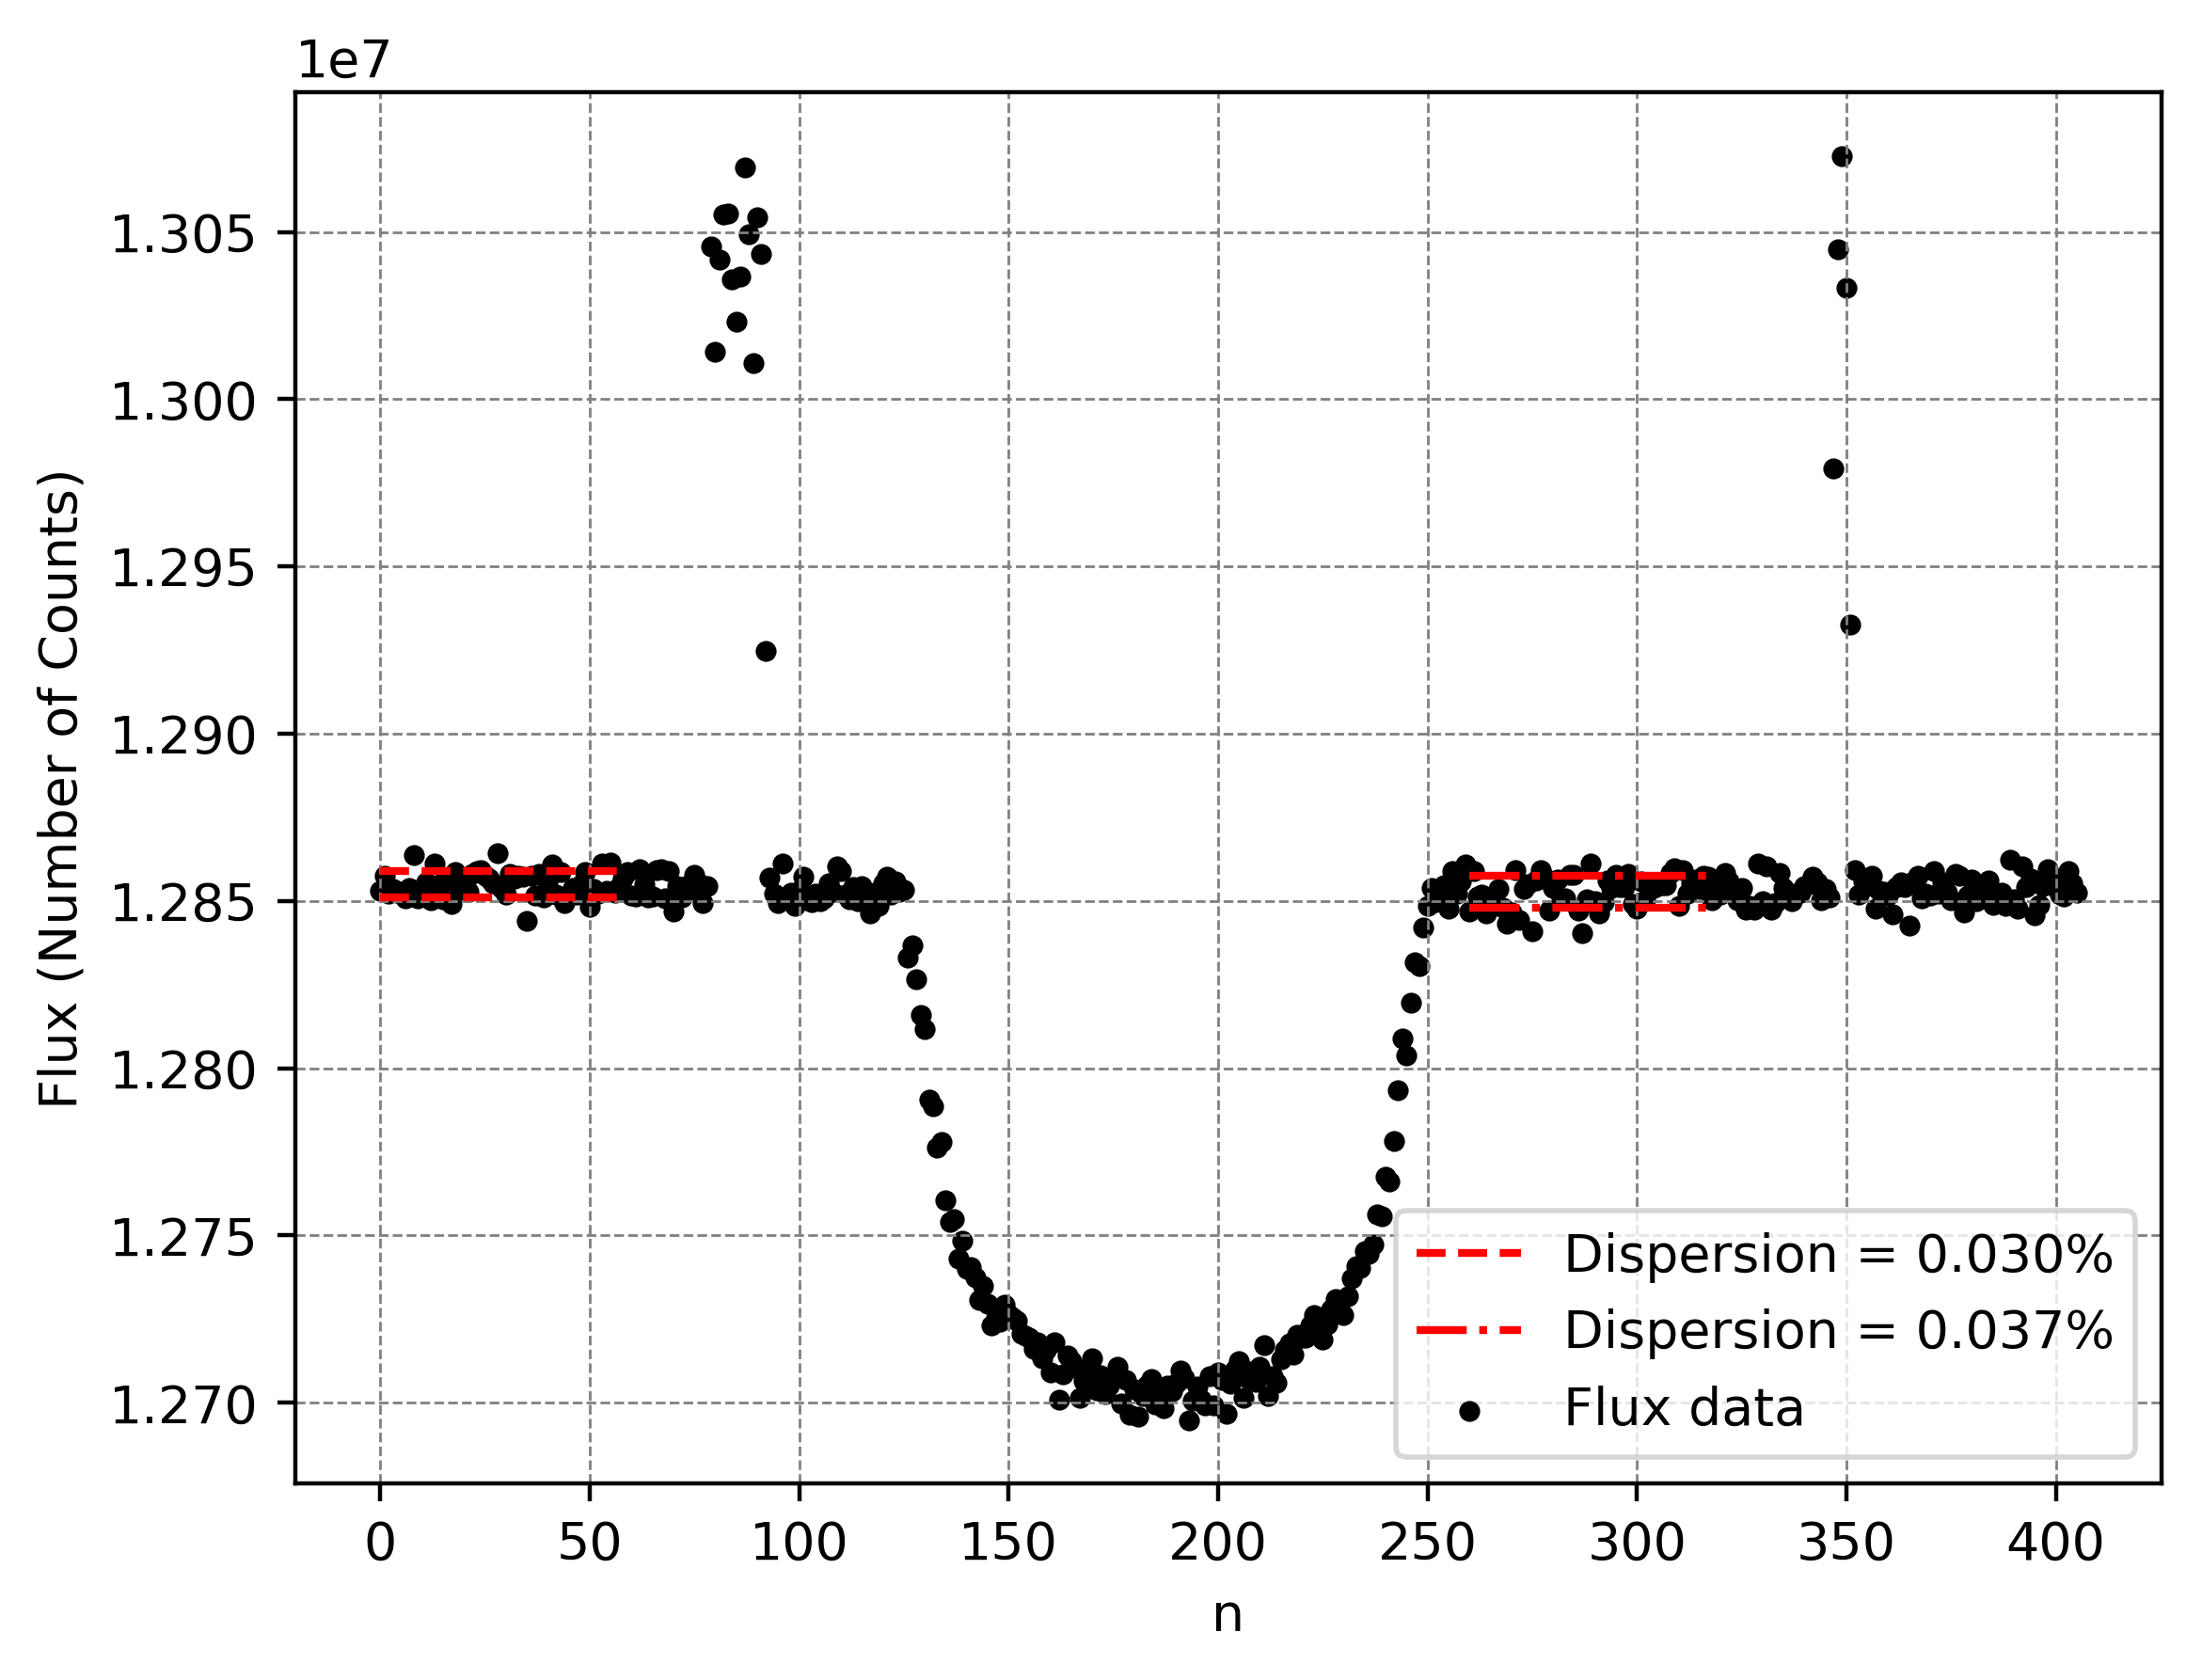
\includegraphics[width=.4\textwidth]{flux.png}
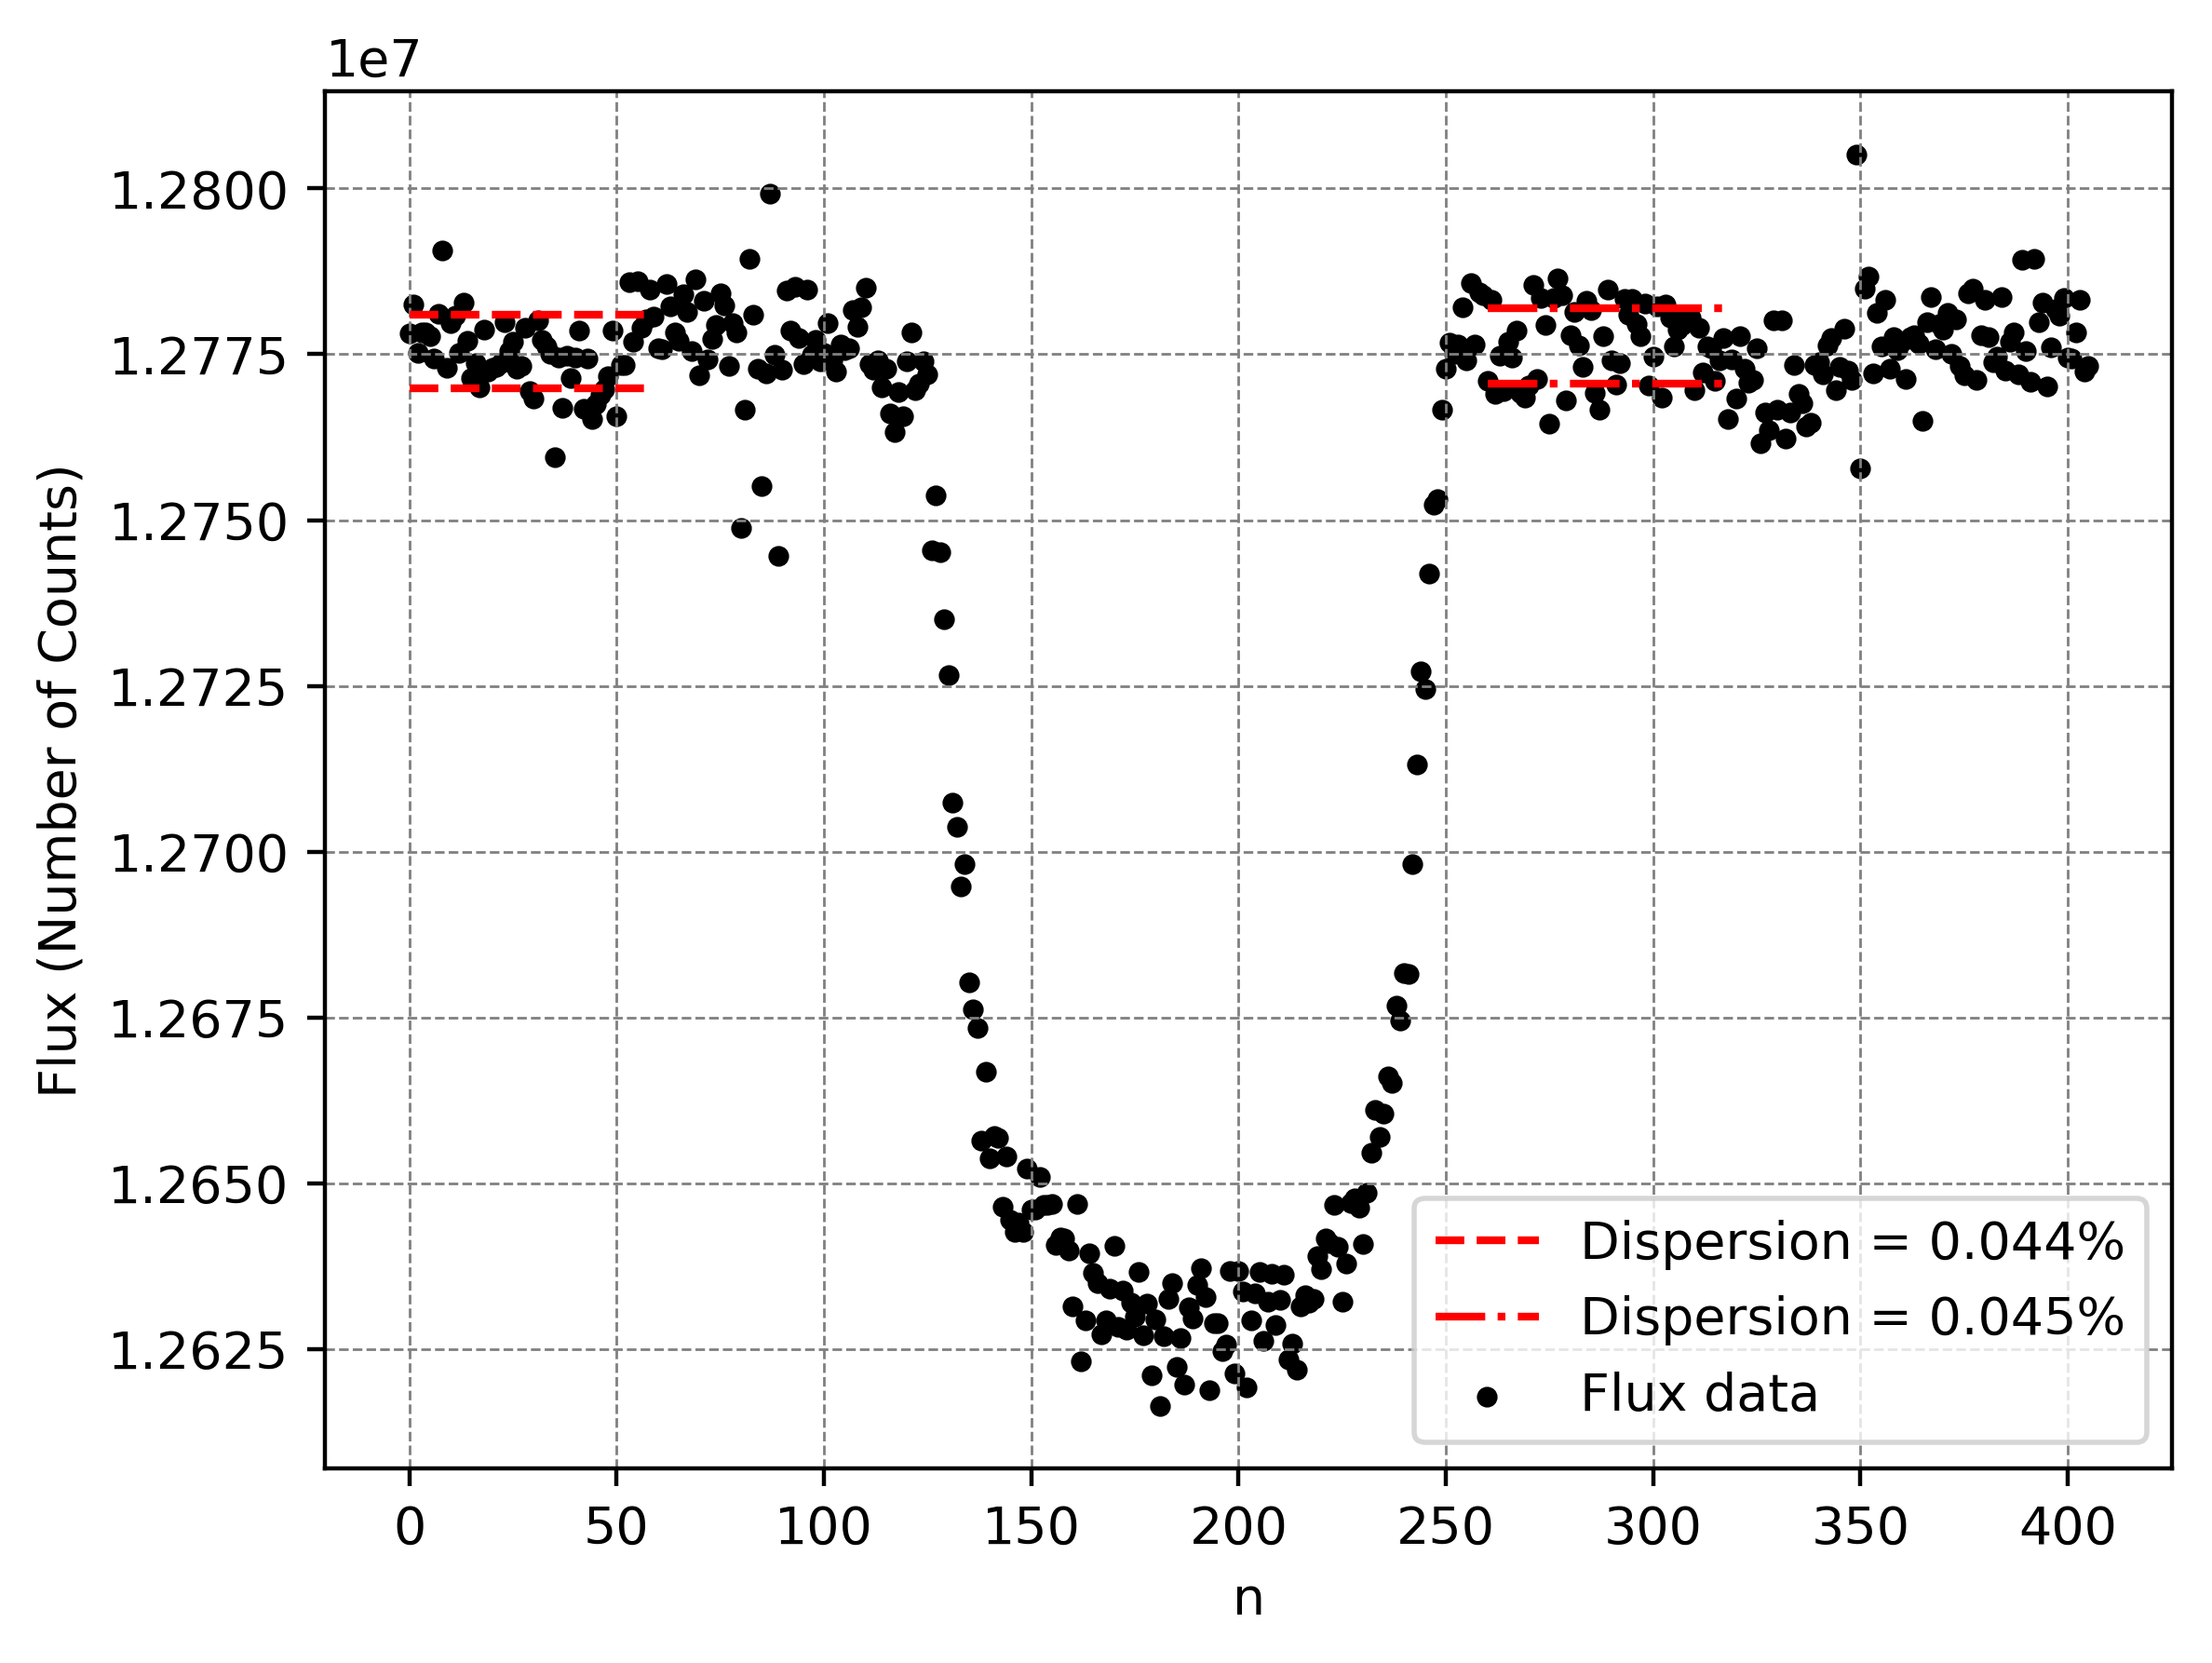
\includegraphics[width=.4\textwidth]{flux_no_avg.png}
\caption{Flux of the target over time. Top: with background mode subtraction; Bottom: both mode and mean subtraction.}
\label{fig:flux}
\end{figure}

The results clearly show a transit happening around the target start by the proeminent well in the flux data. We can also see the effect of the South Atlantic Anomaly on the flux, which raises it as found in the background mean data. By subtracting this mean from the data we can see that this effect is greatly reduced. However, by computing the dispersion,

\begin{equation}
\Delta F = \frac{\sigma_F}{\langle F\rangle}
\end{equation}

of the data in images $[0-60]$ and $[260 - 320]$, we can see that this mean subtraction introduces dispersion in the data.

This dispersion can be used as a figure of merit for the effectiveness of the algorithm. We would ideally want $\lesssim 20$ ppm dispersion in 6 hours of observation to fulfill the CHEOPS mission requirements \cite{cheops}. Since in this case the observation is not that long, we can only estimate the dispersion of the algorithm by computing,

\begin{equation}
\Delta F_{6h} = \frac{\Delta F}{\sqrt{6*60}}
\end{equation}

since $\Delta F$ is for a single minute of observation. By observing Tab. \ref{tab:dispersion}, we can see that the results are similar to those expected, being smaller that 20 when only subtracting the mode and being less than 1 ppm higher than 20 when subtracting the mean.

\begin{table}[]
\centering
\caption{Estimation of the dispersion for 6 hours of observation using the developed method.}
\label{tab:dispersion}
\begin{tabular}{lcccc}
\multicolumn{1}{c}{}                                          & \multicolumn{2}{c}{Mode}       & \multicolumn{2}{c}{Mode + Mean} \\
Images                                                        & {[}0 - 60{]} & {[}260 - 320{]} & {[}0 - 60{]}  & {[}260 - 320{]} \\
\begin{tabular}[c]{@{}l@{}}Dispersion 6h\\ (ppm)\end{tabular} & 15.894       & 19.752          & 20.957        & 20.543         
\end{tabular}
\end{table}

\section{Parameter Optimization} \label{sec:param_opt}

The results in Fig. \ref{fig:flux} were obtained by optimizing the algorithm's parameters in regards to minimizing the dispersion as will be explained in the current section.

We started by optimizing the size of the square for the center of mass computation by setting all other parameters to mere approximations of their optimal value. We can conclude that any value between 20 and 40 would be optimal. We thus chose 20 as the optimal value in order to minimize the number of points used in the calculation and improve computation efficiency.

We proceeded to optimizing the radius of the background calculation. Since this radius limits the area inside which the target is, we would expect that a better background calculation would be the result of a higher value for the radius parameter, thus reducing the dispersion. As expected, we showed that the dispersion tends to reduce for higher values of this parameter. A radius of 25 was chosen for the same reason as before, to reduce the number of points in the calculation while still remaining optimal.

The figures for the optimization of these two parameters are not shown here, but made available as an attachment.

Furthermore, there remained three parameters to optimize, all belonging to the canny edge detection algorithm: $\sigma$ , the higher threshold (T) and the lower threshold (t).

The $\sigma$ parameter controls the radius of the Gaussian filter applied to the image to begin the algorithm. By observing Fig. \ref{fig:sigma_opt} we can see that the dispersion decreases as sigma increases since by applying a larger Gaussian filter we are smoothing the image even more. We choose a value of 1.85 for the optimal $\sigma$ to balance the minimal dispersion with the computed area of the target - too great of sigma and the algorithm finds the wrong edges and the area greatly increases.

\begin{figure}[H]
\centering
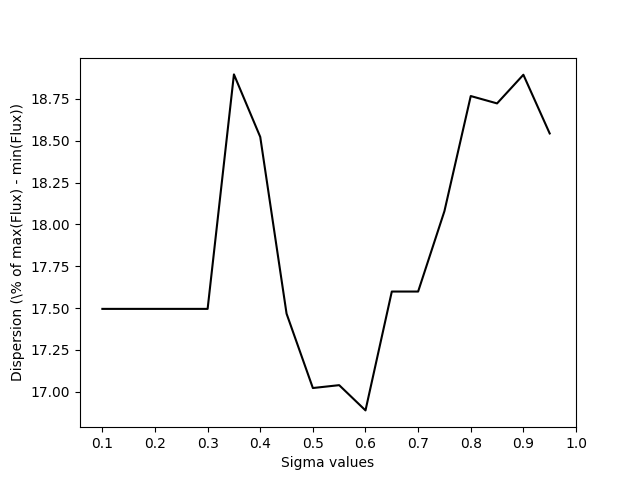
\includegraphics[width=.4\textwidth]{dispersion_sigma.png}
\caption{Dispersion as a function of $\sigma$ for the canny edge detection.}
\label{fig:sigma_opt}
\end{figure}

Using this value of $\sigma$, we optimized T. In Fig. \ref{fig:T_opt} we can see a minimum in the region of 2000 to 4000, with the dispersion greatly increasing for lower and higher values of T. We thus choose T = 3500 by observing the area of the target captured, as for $\sigma$.

\begin{figure}[H]
\centering
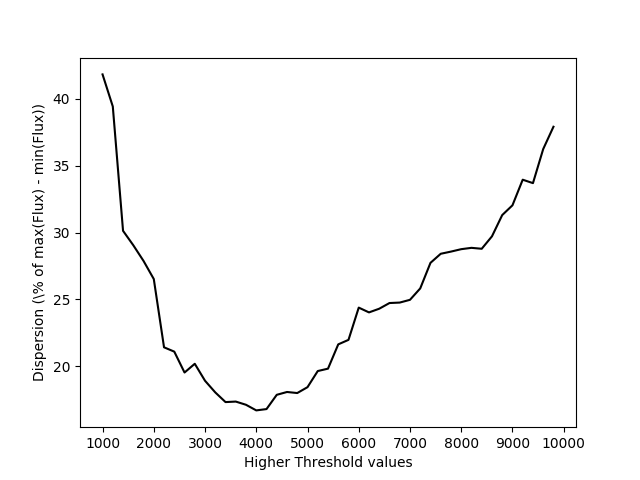
\includegraphics[width=.4\textwidth]{dispersion_T.png}
\caption{Dispersion as a function of T for the canny edge detection.}
\label{fig:T_opt}
\end{figure}

Finally, we computed the lower threshold using all the optimal parameters. The canny edge detection algorithm is expected to be more effective for $t = 0.5T$ thus we are expecting to find a minimum of dispersion for this value. We can see that our expections are met, in Fig. \ref{fig:t_opt}. We thus choose t = 0.5T as the optimal parameter.

\begin{figure}
\centering
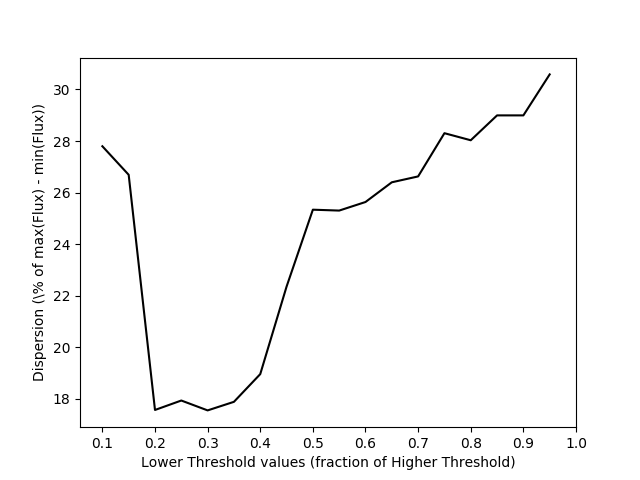
\includegraphics[width=.4\textwidth]{dispersion_t.png}
\caption{Dispersion as a function of t for the canny edge detection.}
\label{fig:t_opt}
\end{figure}

The optimal parameters are presented in Tab. \ref{tab:optimal} for convinience.

\begin{table}[]
\centering
\caption{Optimal algorithm parameters.}
\label{tab:optimal}
\begin{tabular}{ccccc}
\begin{tabular}[c]{@{}c@{}}CM\\ Square Side\end{tabular} & \begin{tabular}[c]{@{}c@{}}Background\\ Radius\end{tabular} & $\sigma$ & T    & t    \\
20                                                       & 25                                                          & 1.85     & 3500 & 0.5T
\end{tabular}
\end{table}

\section{Timing Optimization}

Even though no timing optimization was performed for this algorithm, we can see that it behaves quite well for the studied data.

The pipeline takes approximately 3 secs to produce the flux data with less than a second more to export flux, background mean and background average results.

\section{Conclusions}

%   \begin{enumerate}
%      \item conclusion 1
%      \item conclusion 2
%   \end{enumerate}

%\begin{acknowledgements}
%      Part of this work was supported by the German
%      \emph{Deut\-sche For\-schungs\-ge\-mein\-schaft, DFG\/} project
%      number Ts~17/2--1.
%\end{acknowledgements}

%                                     Two column figure (place early!)
%______________________________________________ Gamma_1 (lg rho, lg e)
%   \begin{figure*}
%   \centering
   %%%\includegraphics{empty.eps}
   %%%\includegraphics{empty.eps}
   %%%\includegraphics{empty.eps}
%   \caption{Adiabatic exponent $\Gamma_1$.
%               $\Gamma_1$ is plotted as a function of
%               $\lg$ internal energy $\mathrm{[erg\,g^{-1}]}$ and $\lg$
%               density $\mathrm{[g\,cm^{-3}]}$.}
%              \label{FigGam}%
%    \end{figure*}
%

%
%                                                One column figure
%----------------------------------------------------------- S_vib
%   \begin{figure}
%   \centering
   %%%\includegraphics[width=3cm]{empty.eps}
%      \caption{Vibrational stability equation of state
%               $S_{\mathrm{vib}}(\lg e, \lg \rho)$.
%               $>0$ means vibrational stability.
%              }
%         \label{FigVibStab}
%   \end{figure}
%
%______________________________________________________________


% WARNING
%-------------------------------------------------------------------
% Please note that we have included the references to the file aa.dem in
% order to compile it, but we ask you to:
%
% - use BibTeX with the regular commands:
%   \bibliographystyle{aa} % style aa.bst
%   \bibliography{Yourfile} % your references Yourfile.bib
%
% - join the .bib files when you upload your source files
%-------------------------------------------------------------------

\begin{thebibliography}{}

\bibitem[(Canny 1986)]{canny} Canny, J. 1986,
      in IEEE Transactions on Pattern Analysis and Machine Intelligence

\bibitem[(CHEOPS Status)]{cheops} Benz, W. , 
      Review of CHEOPS mission and status update

\end{thebibliography}

\end{document}